	In this chapter, we will take a step back and look at primal-dual algorithms in more generality. 
	The goal will be to describe a method of solving a set of primal-dual algorithms for 
	\emph{network design problems}. 
	
	Again we will restrict our attention to bipartite 
	graphs. In network design problems we are given a graph $G = (U,V,E)$ 
	and a cost $c_{uv}$ for each edge $(u,v)\in E$, and the goal is to find a minimum- or maximum-
	cost subset 
	$E\' \subset E$ that satisfies some criteria. Our maximum-weight matching problem is an example
	of this.
\begin{section}{The Classical Primal-Dual Method}
	We begin by looking at what is known as the ``classical'' primal-dual method, which is concerned 
	with linear programs for polynomial-time solvable optimization problems.

	Let us consider the linear program
	\begin{alignat}{2}
		& \text{minimize} & \mathbf{c}^{T}\mathbf{x} \\
		& \text{subject to } & A\mathbf{x} & \geq \mathbf{b} \\
		&& \mathbf{x} & \geq 0
	\end{alignat}
	and its dual
	\begin{alignat}{2}
		& \text{maximize} & \mathbf{b}^{T}\mathbf{y} \\
		& \text{subject to } & A^{T}\mathbf{y} & \leq \mathbf{c} \\
		&& \mathbf{y} & \geq 0.
	\end{alignat}
	We first define a concept that has been subtly at work throughout this thesis. 
	\begin{definition}{(Complementary slackness)}
		Given two linear programs in the form above, the \emph{primal complementary slackness 
		conditions} are the conditions which, given primal solution $\mathbf{x}$, 
		are necessary for a dual solution $\mathbf{y}$:
		\[
			x_j > 0 \implies A^{j}\mathbf{y} = c_j,
		\]
		where $A^{j}$ is the $j$th column of $A$. Similarly, the \emph{dual complementary 
		slackness conditions} are the conditions which, given dual solution $\mathbf{y}$, are 
		necessary for a primal solution $\mathbf{x}$:
		\[
			y_i > 0 \implies A_i\mathbf{x} = b_i,
		\]
		where $A_i$ is the $i$th row of $A$. 
		
		Together, these conditions give us necessary and 
		sufficient conditions for solving the primal-dual system, which we will prove. The 
		(maximization) primal slackness variables are given by 
		$\mathbf{s} = \mathbf{b} - A\mathbf{x}$. The dual slackness variables are given by 
		$\mathbf{t} = A^{T}\mathbf{y} - \mathbf{c}$.
	\end{definition}
	\begin{theorem}
		Let $\mathbf{x}$ be a primal feasible solution, and $\mathbf{y}$ a dual feasible 
		solution. Let $\mathbf{s}$ and $\mathbf{t}$ be the corresponding slackness variables. 
		Then $\mathbf{x}$ and $\mathbf{y}$ are optimal solutions if and only if the following 
		two conditions hold:
		\begin{align}
			x_jt_j &= 0 \quad \text{for all } j \\
			y_is_i &= 0 \quad \text{for all } i
		\end{align}
	\end{theorem}
	\begin{proof}
		Let $u_i = y_is_i$ and $v_j = x_jt_j$, and $\mathbf{u} = \sum_i u_i$, 
		$\mathbf{v} = \sum_j v_j$. Then $\mathbf{u} = 0$ and $\mathbf{v} = 0$ if and only if 
		(7) and (8) hold. Also, 
		\begin{align*}
			\mathbf{u} + \mathbf{v} &= \sum y_is_i + \sum x_jt_j \\
						&= \sum y_i(b_i - A_ix_i) + \sum x_j (A^{T}_jy_j-c_j)\\
						&= \sum b_iy_i - \sum c_jx_j,
		\end{align*}
		so we get that $c^{T}\mathbf{x} = b^{T}\mathbf{y}$ if and only if $u + v = 0$, which 
		proves the statement.	
	\end{proof}
	The general ``tug-of-war'' between the primal and dual suggests an economic interpretation 
	of slackness conditions. We can think of our primal (maximization) problem as concerned with 
	profit given some constraints on resources, i.e. a resource allocation problem. 
	
	The dual can 
	be interpreted as a valuation of the resources -- it tells us the availability of a resource, 
	and its price. So if we have optimal $\mathbf{x}$ and $\mathbf{y}$, we can interpret 
	slackness as follows: if there is slack in a constrained primal resource $i$ ($s_i > 0$), 
	then additional units of that resource must have no value ($y_i = 0$); if there is slack 
	in the dual price constraint ($t_j > 0$) there must be a shortage of that resource ($x_j = 0$).

	We now give an example of complementary slackness in action. Let's look back to our maximum 
	weight matching problem. Recall the primal linear program for maximum-weight matching:
	%Maximum matching ILP%
	\begin{alignat}{3}
		& \text{maximize } & \sum_{u,v} c_{uv} x_{uv}& \\
		& \text{subject to } \quad & \sum_{v} x_{uv} & \leq 1, & \quad \forall u\in U&, \\
				     &\quad & \sum_{u} x_{uv} & \leq 1, & \quad \forall v\in V &, \\
				&& x_{uv} & \geq 0.
	\end{alignat}
	and its dual
	%Vertex cover ILP%
	\begin{alignat}{3}
		& \text{minimize } & \sum_u y_u + \sum_v y_v& \\
		& \text{subject to } \quad & y_u + y_v & \geq c_{uv}, & \quad \forall 
					u\in U,\ v\in V &, \\
				    && y_u,y_v & \geq 0.
	\end{alignat}
	The format here is a little different, since our primal is a maximization problem and the dual 
	is a minimization, but it's easy enough to reverse the roles. It's easy to see our 
	corresponding primal complementary slackness conditions are
	\begin{equation}
		x_{uv} > 0 \implies y_u + y_v = c_{uv}.
	\end{equation}
	The dual complementary slackness conditions are
	\begin{align}
		y_u > 0 &\implies \sum_v x_{uv} = 1,\\
		y_v > 0 &\implies \sum_u x_{uv} = 1.
	\end{align}
	In general, the slackness conditions guide us in our algorithm -- they tells us how, given a 
	solution to one of the problems, we should augment the solution to the other. For example, the 
	algorithm we presented for maximum-weight matching/minimum vertex cover intializes with 
	a solution to both the primal and dual that satisfies conditions (8) and (10); the algorithm 
	then at each step works to decrease the number of conditions in (9) that are unsatisfied, while 
	maintaining satisfiability of (8) and (10). This method is not unique to the Hungarian 
	algorithm. In fact, the Hungarian algorithm paved the way for this general method, which we 
	describe presently.

	Looking back at the original linear programs at the beginning of this chapter, suppose we have 
	a dual feasible solution $\mathbf{y}$. We can then state the problem of finding a feasible 
	primal solution $\mathbf{x}$ that obeys our complementary slackness conditions as another 
	\emph{restricted} linear program. Define the sets $A = \{j\ |\ A^{j}\mathbf{y} = c_j\}$ and 
	$B = \{i\ |\ y_i = 0\}$. So $A$ tells us which dual constraints (5) are tight, 
	given the solution $\mathbf{y}$, and $B$ tells us which $y_i$ are 0. What we want to do is 
	give a linear program to find a solution $\mathbf{x}$ that minimizes the 
	``violation'' of the complementary slackness conditions and the primal constraints, and to do 
	so we will index our variables by these sets. We will 
	have slack variables $s_i$ which will describe the difference between $A_i\mathbf{x}$ and $b_i$ 
	for $i\notin A$. We do this because we want to look at all $y_i > 0$ where the we do not 
	have that $A_i\mathbf{x} = b_i$. So part of our objective function will be to minimize the 
	sum of these $s_i$. We also want to minimize the sum over variables $x_j$ where $j\notin A$. 
	This is because we want to see if there are any $x_j$ such that $A^{j}\mathbf{y} \neq c_j$. 
	So we give the following restricted primal linear program:
	\begin{alignat}{3}
		& \text{minimize } & \sum_{i\notin B} s_i + \sum_{j\notin A} x_j & \\
		& \text{subject to } & A_i\mathbf{x} & \geq b_i, & \quad i\in B &, \\
				     && A_i\mathbf{x} - b_i & = s_i, & \quad i\notin B &, \\
				     && \mathbf{x} & \geq 0, \\
				     && \mathbf{s} & \geq 0.
	\end{alignat}
	Observe that if this restricted primal has a feasible solution $(\mathbf{x},\mathbf{s})$ such 
	that the objective function is 0, then $\mathbf{x}$ is a feasible primal solution that 
	satisfies the complementary slackness conditions for the dual solution $\mathbf{y}$. This 
	means that $\mathbf{x}$ and $\mathbf{y}$ are optimal primal and dual solutions. If, however, 
	the optimal solution to this restricted primal has value greater than 0, more work is required. 
	We can consider the dual of the restricted primal:
	\begin{alignat}{3}
		& \text{maximize } & \mathbf{b}^{T}\mathbf{w} & \\
		& \text{subject to } & A^{j}\mathbf{w} & \leq 0, & \quad j\in A &, \\
				     && A^{j}\mathbf{w} & \leq 1, & \quad j\notin A &, \\
				     && w_i\' & \geq -1, & \quad i\notin B &, \\
				     && w_i\' & \geq 0. & \quad i\in B &.
	\end{alignat}
	What we want here is to improve our dual solution. By assumption, the optimal solution to this 
	linear program's primal is greater than 0, so we know that this dual has a solution 
	$\mathbf{w}$ such that $\mathbf{b}^{T}\mathbf{w} > 0$. What we want is the existence of 
	some $\epsilon > 0$ such that $\mathbf{y}^{'} = \mathbf{y} + \epsilon \mathbf{w}$ is a 
	feasible dual solution. In particular, a solution of this form will be an improvement on our 
	original solution $\mathbf{y}$. We can calculate bounds on $\epsilon$ as follows. The two 
	conditions we must satisfy in order to maintain dual feasibility are that $y^{'} \geq 0$ and 
	$A^{T}y^{'} \leq c$. This means that we need 
	\begin{align}
		y_i + \epsilon w_i &\geq 0 \\
		A^{T}_j y + A^T_j \epsilon w & \leq c_j.
	\end{align}
	Let's consider the first one. When $w_i > 0$, we are fine; we need to be careful when 
	$w_i < 0$ since this could potentially violate the inequality. Solving in this way, we get 
	a first bound on $\epsilon$:
	\[
		\epsilon \leq \min_{i\in B: w_i < 0} (-y_i/w_i).
	\]
	Now let's address the second inequality. When $A^{T}_jw \leq 0$, we are defintely okay. We 
	need to be careful about violating the constraint when $A^{T}w > 0$. Thus, we can calculate a 
	second bound on $\epsilon$:
	\[
		\epsilon \leq \min_{j\in A: A^{T}_jw > 0} \frac{c_j-A^{T}_jy}{A^{T}_j w}.
	\]
	If we choose the lower of these two $\epsilon$ values, we obtain a new feasible dual solution 
	that has greater objective value. We can then work by reiterating the procedure, with the hope 
	that we find an optimal primal solution.

	It's not immediately clear why reducing our original linear programs to a series of linear 
	programs is heplful. However,  note that the vector $\mathbf{c}$ has totally disappeared in 
	the restricted primal and its dual. Recall that in the original linear program, $\mathbf{c}$ 
	gave us the edge-costs on our graph. So this method reworks our original weighted problem 
	into unweighted parts, which are easier to solve. Oftentimes, it is the case that 
	we can interpret these unweighted problems as purely combinatorial problems, which means that 
	instead of actually solving the problem with linear programming, we can solve it by 
	combinatorial 
	methods. Using a combinatorial algorithm to find a solution $\mathbf{x}$ that obeys the 
	complementary slackness conditions, or to find an improved dual solution $\mathbf{y}$, is 
	oftentimes more efficient.
\end{section}
	
\begin{section}{The Primal-Dual Method for Weighted Matchings}
	Let us now look at an example of this method. We will look at a weighted matching problem, as 
	in the previous chapter, but this time we will look at \emph{minimizing} the cost of the 
	matching, instead of maximizing. We do this mainly because it illustrates something important 
	about the underlying structure of these matching problems. It will be easy to see how the 
	same method can be used for the case in which we want a maximimum matching. So the primal 
	linear program for a minimum weight perfect matching on a bipartite graph is given as follows. 
	\begin{alignat}{3}
		& \text{minimize } & \sum_{u,v} c_{uv} x_{uv}& \\
		& \text{subject to } \quad & \sum_{v} x_{uv} & \geq 1, & \quad \text{for all } u\in U& \\
				     &\quad & \sum_{u} x_{uv} & \geq 1, & \quad \text{for all } v\in 
				     V & \\
				&& x_{uv} & \geq 0.
	\end{alignat}
	Its dual is
	\begin{alignat}{3}
		& \text{maximize } & \sum_{u}y_u + \sum_{v}y_v & \\
		& \text{subject to } \quad & y_u + y_v & \leq c_{uv}, & \quad \text{for all }
					u\in U,\ v\in V & \\
				    && y_u,y_v & \geq 0.
	\end{alignat}
	We need to start with a dual feasible solution, and try to find a primal solution that 
	minimizes the violation of the constraints and slackness conditions. We can start with the 
	trivial dual solution of $y_u,y_v = 0$ for all $u,v$. Let's now think about our primal 
	complementary slackness. The set $A$ is given by $\{(u,v)\in E\ :\ y_u + y_v = c_{uv}\}$. 
	We know that these are the edges we want to include in our matching, and since we know our 
	linear program has integer solutions at extreme points of the polyhedron, let's specify that 
	$x_{uv} = 0$ for $(u,v)\notin a$. Now, our other slackness variables $s_u,s_v$ look like 
	\begin{align*}
		\sum_{v:(u,v)\in E} x_{uv} - s_u &= 1 \\
		\sum_{u:(u,v)\in E} x_{uv} - s_v &= 1.
	\end{align*}
	So we want to minimize over the sum of $s_u$ and $s_v$. Note that at this point, our set $B$ 
	consists of all vertices. So our restricted primal linear program is
	\begin{alignat}{3}
		& \text{minimize } & \sum_{u\in U} s_u + \sum_{v\in v} s_v & \\
		& \text{subject to } & \sum_v x_{uv}, - s_u & = 1 & \quad \text{for all } u & \\
				     && \sum_u x_{uv}, - s_v & = 1 & \quad \text{for all } v & \\
				     && x_{uv} & = 0, & \quad (u,v)\notin A \\
				     && x_{uv} & \geq 0, & \quad (u,v)\in A \\
				     && \mathbf{s} & \geq 0.
	\end{alignat}
	Let's first observe that all components of this restricted primal take on values 0 or 1, as 
	in the original primal. Moreover, note that we have turned a weighted problem into an 
	unweighted combinatorial problem. We've specified that we are not including any edge 
	$(u,v)\notin A$ in our matching, and we are trying to include as many $(u,v)\in A$ as possible 
	in our matching by minimizing the slackness variables. Note that the graph $G^{'} = (U,V,J)$ 
	is exactly the equality subgraph as defined in the previous chapter! In our Hungarian algorithm 
	we repeatedly sought to find maximum cardinality matchings within this subgraph, which is 
	exactly what this restricted primal is having us do. This tells us that the problems of maximum 
	weight matching and minimum weight matching only differ in the labeling we are specifying. The 
	underlying procedure for solving both of the problems is essentially the same. So if we find a 
	perfect matching in $G^{'}$, we will have found an $\mathbf{x}$ that obeys the complementary 
	slackness conditions, i.e. $\sum_u s_u + \sum_v s_v = 0$. Moreover, this implies that the 
	dual solution $\sum_u y_u + \sum_v y_v$ must be optimal as well.\\
	Now, if the solution $\sum_u s_u + \sum_v s_v > 0$, we do not have an optimal $\mathbf{x}$, 
	so we need to adjust our dual. We look at this now, in the dual linear program of the 
	restricted primal:
	\begin{alignat}{3}
		& \text{maximize } & \sum_{u\in U} w_u + \sum_{v\in V} w_v & \\
		& \text{subject to } & w_u + w_v & \leq 0, & \quad \text{for all } (u,v)\in A & \\
				     && w_u + w_v & \leq 1, & \quad \text{for all } (u,v)\notin A & \\
				     && w_u,w_v & \geq -1, & \text{for all } u,v\notin B \\
				     && w_u,w_v & \geq 0, & \text{for all } u,v\in B \\
				     && \mathbf{w} & \geq 0.
	\end{alignat}
	We now want to find an $\epsilon$ such that the solution $z = \sum_u y_u + \sum_v y_v + 
	\epsilon (\sum_u w_u + \sum_v w_v)$ is (1) feasible and (2) an improvement of the dual 
	objective. First of all, we know that since the restricted primal has solution $\geq 0$, 
	the solution to this dual will also be $\geq 0$. So we just need to worry about the condition 
	\[
		y_u + y_v + \epsilon (w_u + w_v) \leq c_{uv}.
	\]
	So we get that we at least need that $\epsilon \leq \min_{(u,v)\notin A: w_u + w_v > 0}
	\frac{c_{uv} - y_u - y_v}{w_u + w_v}$. We can refine this by noting that since 
	$0 < w_u + w_v \leq 1$ for $(u,v)\notin A$, we have $\epsilon = \min_{(u,v)\notin A} 
	(c_{uv} - y_u - y_v)$. Note that the negative of this is exactly the quantity we modify our 
	labeling by in the Hungarian algorithm in the previous chapter. Thus we've found an 
	$\epsilon$ that maintains dual feasibility, and increases the objectie function. We can use 
	this solution and revisit the restricted primal in order to look for an improved feasible 
	primal solution.
\end{section}

\begin{section}{Auction Algorithms}
	We now look at a cool application of weighted bipartite matchings, given by Bertsekas 
	\cite{Bertsekas1992}. Let's imagine our assignment 
	problem is an auction. We will motivate this through an economic lens. Suppose that a good $g$ 
	has a price $p_g$, and a bidder $b$ must pay $p_g$ to receive this item. Suppose that the 
	amount bidder $b$ is willing to pay for good $g$, or $b$'s valuation of $g$, is $c_{bg}$. 
	Then the net value 
	of this item $g$ to bidder $b$ is $c_{bg} - p_g$. Let's also adopt the notation that 
	$A(b)$ is the set of all items bidder $b$ is interested in (willing to pay for). 
	Assuming that each bidder $b$ is a rational agent acting 
	in their own best interest, each bidder $b$ would want to be assigned a good $g^{*}$ that 
	maximizes their net value, i.e. for all bidders $b$ with goods $g^{*}$, we have that 
	\begin{align}
		c_{bg^{*}} - p_{g^{*}} = \max_{g\in A(b)} \{c_{bg} - p_g \}.
	\end{align}
	This would give us an economic system in equilibrium; no bidder would have an incentive to 
	seek/trade for a different good.  

	The reason this is of interest to us is that an equilibrium assignment maximizes total 
	profit (i.e. it solves the primal linear program for maximum weight matchings), while the 
	corresponding set of prices solves an associated dual problem.

	Our goal is to maximize the total amount earned in the auction -- i.e. to 
	maximize $\sum_{(b,g)} c_{bg}$, under the constraint that no bidder gets more than one good, 
	and no good is purchased by more than one bidder.
	It will be useful for us to consider an alternate, but equivalent dual problem, which is 
	suggested by our complementary slackness conditions. For a more detailed treatment of this 
	equivalence, see Bertsimas and Tsitsiklis \cite{bertsimas1997introduction}. 
	In the auction setting, it does not make 
	sense to have a labeling on the vertices in $B$ (the set of buyers) whereas in the usual dual we 
	have variables on both sets of vertices that partition our graph. The usual dual is as 
	follows:
	\begin{alignat}{3}
		& \text{minimize } & \sum_{b=1}^n r_b + \sum_{g=1}^n p_g & \\
		& \text{subject to } & r_b + p_g & \geq c_{bg}, &\quad \text{for all } (b,g)\in E\\
				     && r_b,p_g & \geq 0. & \quad b\in B,\ g\in G
	\end{alignat}
	In the auction setting, only 
	values of $p_g$ make sense; ``prices'' ($r_b$) on the bidders is meaningless (unless our 
	auction is two-way, which we are not considering). 
	Note that $\sum_b r_b$ is minimized (while still maintaining feasibility) when we set each 
	$r_b$ to the largest value allowed by the constraints (4.52), i.e. given $p_{g}$ for 
	$g=1, \dots, n$ , set
	\[
		r_{g} := \max_{g=1,\dots, n} \{c_{bg} - p_g\}.
	\]
	This gives us the following equivalent dual objective function 
	\begin{align}
		&\text{minimize }\{ \sum_b \max_g \{c_{bg} - p_g\} + \sum_g p_g\},
	\end{align}
	which is unconstrained (except for the usual nonnegativity requirement). 
	Note that this is an exact translation of our complementary slackness 
	conditions (4.50). Again, this illustrates the importance of complementary slackness in the 
	creation of algorithms for combinatorial optimization.

	\begin{subsection}{The Naive Algorithm}
		We will first proceed in describing a naive auction algorithm, which although clever, 
		does not always work. Nonetheless, we will use it as motivation for 
		our final auction algorithm.

		Throughout the algorithm, we wil keep track of two sets of bidders -- those that are 
		currently assigned a good $g$, and those that are not. At a general step in our 
		algorithm, we will want to consider a bidder $b$ that is currently not the owner of any 
		good, and find a good $g^{*}$ such that  $c_{bg^{*}} - p_{g^{*}} = \max_{g\in A(b)}  
		\{c_{bg} - p_g\}$. 
		We will then need to do two things: (1), replace the current owner $b^{'}$ of $g^{*}$ 
		(put them back into the set of unassigned bidders) with $b$; (2) bump the price of 
		$g^{*}$ by some amount $\delta_b$. Intuitively, we want to increase $p_{g^{*}}$ by the 
		largest 
		amount while still maintaining the fact that $g^{*}$ offers maximal value to $b$. We can 
		easily accomplish this by setting $\delta_b = v_b - w_b$, where $v_b = \max_{g\in A(b)} 
		\{c_{bg} - p_g\} = p_{g^{*}}$ and $w_b = \max_{g\in A(b),\ g\neq g^{*}} 
		\{c_{bg} - p_g\}$. 
		This simply says that we are bumping the price $p_{g^{*}}$ by the difference in the 
		profit of the best object and the profit of the second best object.

		This is a simple algorithm that has one major problem: there are cases in which it 
		does not terminate. The issue is that the bidding increment $\delta_b$ is zero when 
		more than one object offers maximum value to a bidder $b$. Consequently, a situation may 
		arise in which a number of bidders contend for a smaller number of equally desirable 
		objects, creating an infinite loop. An example of this is shown in Figure 4.1, taken 
		from Bertsekas \cite{Bertsekas1992}.
		\begin{figure}[h]
			\centering
		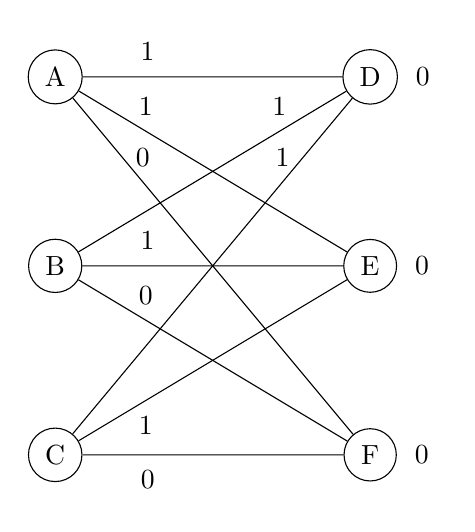
\begin{tikzpicture}[scale=.8,auto=left,every node/.style={circle,draw=black}]
			%left nodes
			\node (n1) at (1,10) {A};
			\node (n2) at (1,7) {B};
			\node (n3) at (1,4) {C};

			%right nodes
			\node [label=right:{0}] (n4) at (6,10) {D};
			\node [label=right:{0}] (n5) at (6, 7) {E};
			\node [label=right:{0}] (n6) at (6, 4) {F};
		
			%edges
			\draw (n1) -- node[near start, draw=none, above] {1} ++ (n4);
			\draw (n1) -- node[near start, draw=none, above] {1} ++ (n5);
			\draw (n1) -- node[near start, draw=none, above] {0} ++ (n6);
			\draw (n2) -- node[near end, draw=none, above] {1} ++ (n4);
			\draw (n2) -- node[near start, draw=none, above] {1} ++ (n5);
			\draw (n2) -- node[near start, draw=none, above] {0} ++ (n6);
			\draw (n3) -- node[near end, draw=none, above] {1} ++ (n4);
			\draw (n3) -- node[near start, draw=none, below] {1} ++ (n5);
			\draw (n3) -- node[near start, draw=none, below] {0} ++ (n6);
		\end{tikzpicture}
			\caption{Example where the naive algorithm does not terminate.} 
		\end{figure}
		In this figure the initial prices on all goods is zero. All bidders desire objects 
		$\mbox{D}$ and $\mbox{E}$ since they offer a benefit of $1-0 = 1$, while object 
		$\mbox{F}$ offers a benefit 
		of zero to all bidders. Say we first assign bidder $\mbox{A}$ to object $\mbox{D}$. 
		Then the algorithm 
		will cycle as bidders $\mbox{B}$ and $\mbox{C}$ compete for item $\mbox{E}$ without 
		its price being raised.

		The issue with our naive algorithm can be remedied by adding a small perturbation term 
		to our complementary slackness, which will break the cycles that cause problems like in 
		Figure 4.1.
	\end{subsection}
	\begin{subsection}{The Auction Algorithm}
		In real auctions it is often the case that each bid for an object must raise the 
		object's price by some minimum positive increment $\epsilon$. 
		This will ensure that no matter what, whenever someone 
		is assigned an item, the price raises by some non-zero amount. We will say that 
		an assignment and a price vector satisfy $\epsilon$-\emph{complementary 
		slackness} if 
		\begin{align}
			& c_{bg^{*}} - p_{g^{*}} \geq \max_{g\in A(b)} \{c_{bg} - p_g\} - \epsilon.
		\end{align}
		The new auction algorithm will be the same as the naive one, except in the way we 
		adjust prices; now $\delta_b := v_b - w_b + \epsilon$. We give the pseudocode below. We 
		will use a data structure called a queue, denoted $\mathcal{Q}$, to keep track of 
		unassigned bidders. A queue works exactly how one might think: new elements are placed 
		at the ``end,'' or enqueued, and members are removed from the ``top,'' or dequeued.
		\begin{figure}[h]
		\begin{center}
			\begin{minipage}{3in}
			\begin{codebox}
				\Procname{$\proc{Auction Algorithm} (B,G,E,c)$}
				\li For each $g\in G$, set $p_g \gets 0$
				\li Queue $\mathcal{Q} \gets B$.
				\li \While $\mathcal{Q}\neq \emptyset$
					\Do
				\li		$b = \mathcal{Q}.deque()$
				\li		Find $g^{*}\in A(b)$ that maximizes $c_{bg} - p_{g}$
				\li		Let $b^{'}$ be the bidder currently assigned to $g^{*}$ 
				(\emph{null} if none)
				\li		\If $c_{bg^{*}} - p_{g^{*}} \geq 0$
							\Then
				\li				$\mathcal{Q}.enqueue(b^{'})$
				\li				Assign $g^{*}$ to $b$
				\li				$p_g^{*} = p_g^{*} + \delta_b$
							\End
					\End
				\li \Return Assignment and price vector
			\end{codebox}
			\end{minipage}
			\caption{Pseudocode for the auction algorithm}
		\end{center}
		\end{figure}
		We first discuss why this algorithm terminates. 
		The first thing we should note is that once all goods 
		receive a bid the algorithm is done, since each person bids on the good they 
		currently desire most. Now, suppose there is some good that receives $k$ bids. This will 
		increase the good of this price by at least $k\epsilon$. Clearly there is some $k$ for 
		which the good is less desirable than some other good that has not received any bids 
		thus far. So it must be the case that a good can only receive a finite number of 
		bids before it is considered inferior to some other good that has not been bid on. For 
		the case in which our graph is not fully dense, see Bertsekas \cite{Bertsekas1992}, 
		Appendix 2.
	
		Now we need to discuss how satisfying $\epsilon$-complementary slackness affects our 
		solutions. Because we are relaxing our original complementary slackness constraint, 
		we should not in general expect to get optimal solutions. 
		In fact, optimality of our solution relies entirely on 
		how we choose our $\epsilon$. It turns out that whatever $\epsilon$ is, 
		an assignment of bidders and a price vector that together satisfy $\epsilon$-
		complementary slackness will be within $n\epsilon$ of optimal. We state this formally.
		\begin{theorem}
			A feasible assignment of bidders along with a price vector $\mathbf{p}$, 
			which together satisfy $\epsilon$-complementary slackness, 
			is within $n\epsilon$ of being optimal. 
			Furthermore, the price vector is within $n\epsilon$ of being an optimal dual 
			solution.
		\end{theorem}
		\begin{proof}
			Let $\Gamma$ be the value of a total optimal assignment, and $\Omega$ the 
			corresponding dual cost. So 
			\begin{align}
				\Gamma &= \max_{g^{*}\in A(b)} \sum_b c_{bg} \\
				\Omega &= \min_{p_g} \{\sum_b \max_{g\in A(b)} \{c_{bg} - p_g\} + 
				\sum_g p_g\},
			\end{align}
			where in (4.56) we specify that no good is assigned to two bidders, and no bidder 
			is assigned to two goods.

			Firstly, weak duality tells us that $\Gamma \leq \Omega$. Since our assignment 
			and prices satisfy $\epsilon$-complementary slackness, we know that 
			\[
				\max_{g\in A(b)} \{c_{bg} - p_g\} - \epsilon \leq c_{bg^{*}} - p_{g^{*}}.
			\]
			This means that we have 
			\[
				\Omega \leq \sum_b \left(\max_{g\in A(b)} \{c_{bg} - p_g\} + p_{g^{*}} 
				\right) \leq \sum_b c_{bg^{*}} + n\epsilon \leq \Gamma + n\epsilon.
			\]
			This shows that both our primal and dual objective functions are within 
			$n\epsilon$ of optimality.
		\end{proof}
		Note that in the case where all $c_{bg}$ are integers (which is usually the case in 
		auctions), choosing an $\epsilon < 1/n$, gives an optimal output for both the primal 
		and dual solutions.
\end{subsection}
\end{section}
\begin{section}{Concluding Remarks}
The primal-dual method described in this chapter is just a glimpse into what is a fruitful area of 
active research. Ultimately, the goal is to use this method to develop approximation algorithms 
for problems known to be NP-hard. Unfortunately, we did not have the time to thoroughly explore 
this facet in this thesis. However, this thesis provides an introduction to the method so that 
perhaps in the future some dilligent student may look into this method as it applies to problems in NP.
\end{section}
